\documentclass[../main.tex]{subfiles}
 
\begin{document}

\section{Sunday}

Today is your first shift as a student volunteer. You show up to check in with your Team Leader, who will be responsible for placing you somewhere in the masive \textit{Experience Hall} with one of the vendors. Experience Hall is dark as you walk in through one of the dozen or so doors leading into the room. The first thing you see is a seating area where people with couches scattered across a large rug. Then there is a barricade of Student volunteers standing an arms width apart to visully inspect badges walking by them. Remember, these badges are expensive and anyone can walk into the main lobby off the street. Beyond this barricade is a labyrinth of vendors with black curtains between stations and black tablecloths covered with posters, handouts, business cards, and whatever demo equipment each vendor has brought. On either side of a booth is a large poster illuminated from beneath by a spotlight which provides an abstract for what you are looking at.

You express an interest in haptic technology as your pack of SVs lead throughout the showroom like flock of geese by your leader. You are checked off on the clipboard for your first shift and introduced to couple of researchers from the Koji-Lab. This lab is based out of the University of Electro-Communications in Tokyo, Japan. Quickly, you realize your chief responsibilities will be greeting attendees who walk by, encouraging them to try the technology laying on the table alongside you as you explain the gist of the pamphlets being handed out. The researchers do not speak english very well.

What this particular team has brought to the convention center is a device which attempts to produce sensations of texture as you move your virtual hand through a Unity simulation. Before you can begin explaining the demonstration to curious attendees, you must try it out for yourself. The researchers carefully tuck your thumb, index, and middle finger into sensors in the way a finger pulse oximeter is usually clamped to a digit. In front of you is a monitor showing a real-time rendering of a wooden desk covered with a book, a metal grate with ribs and spirals, a Poké Ball, a pencil, a translucent ball, and a wooden cube next to a square hole. You see an outstretched hand that moves with yours as you push a platform serving as a mouse. The platform that has been built around a mouse is designed to hold your hand with your palm down and fingers outstretched, as if you are trying to hover over the virtual objects on the virtual desk without picking them up.

\begin{figure}[h!]
	\centering
	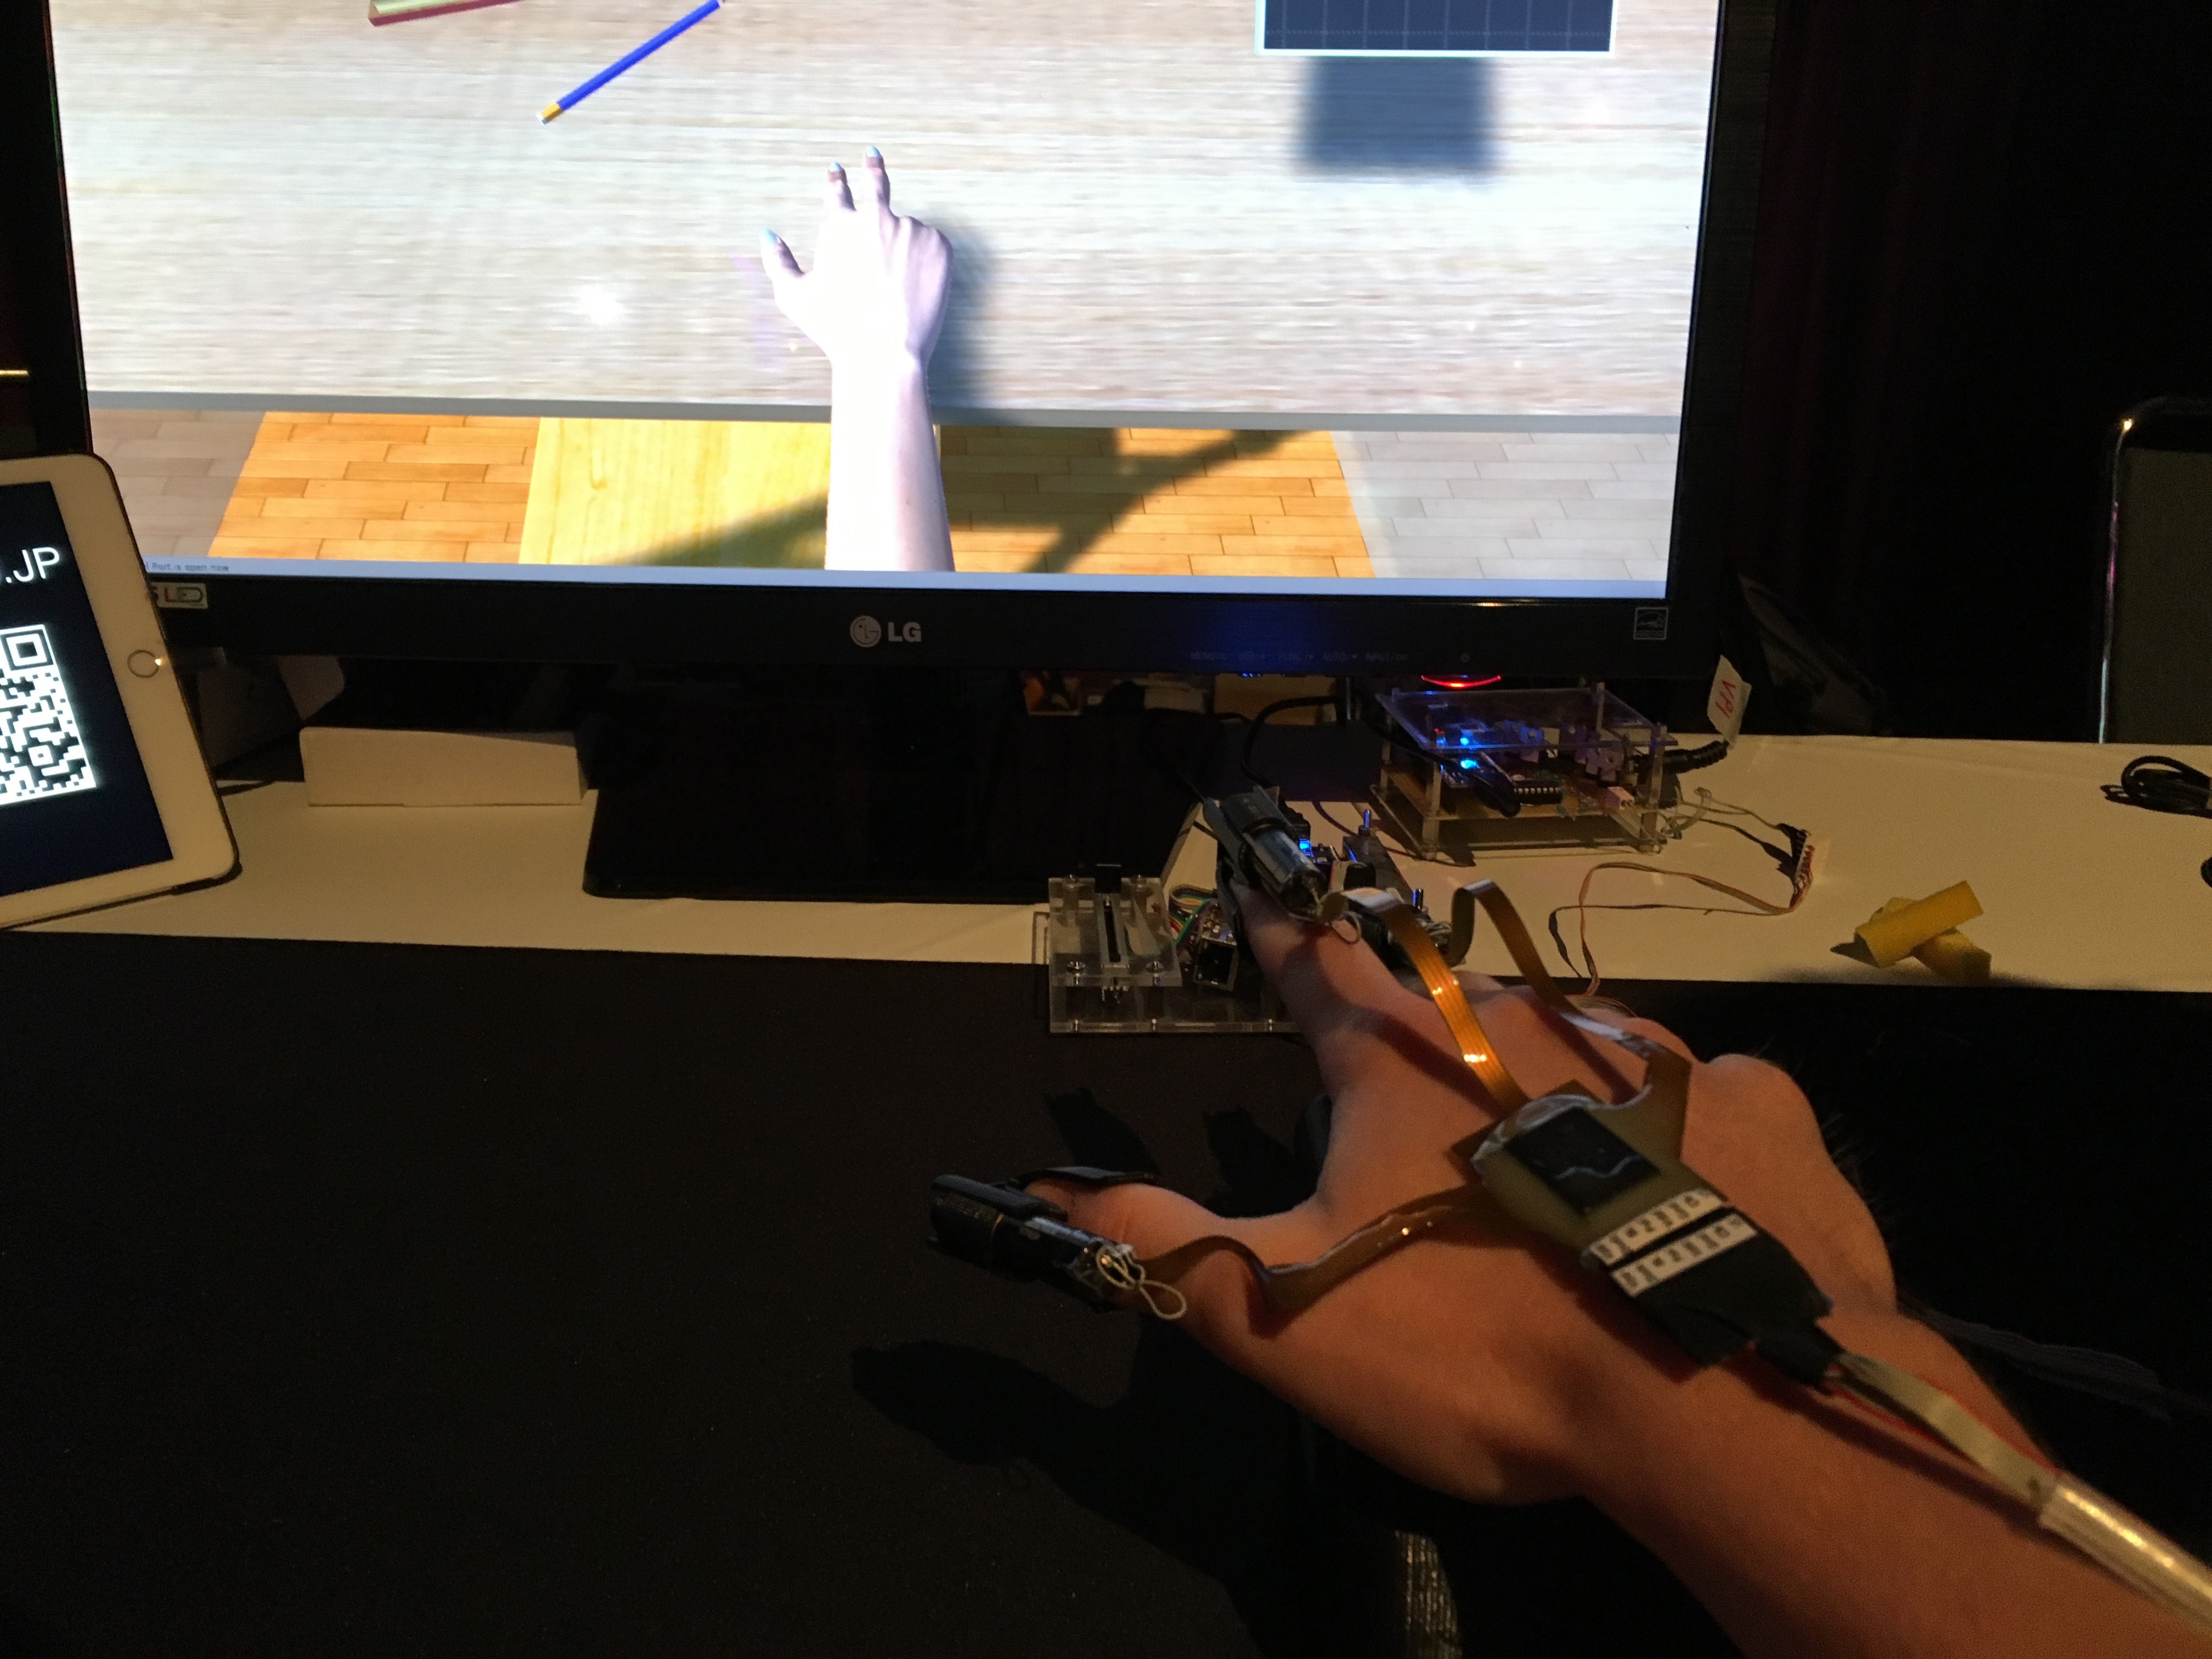
\includegraphics[width=\textwidth]{fingar}
	\caption*{The University of Electro-Communications in Tokyo, Japan contributed to serveral booths during SIGGRAPH 2016.}
\end{figure}

After calibrating the device attached to your fingers, you begin moving your hand (and your virutal fingers) about the scene, the high and low vibrations and small electrical current tricking your fingers into sensations of texture. It was not without some trepidation that you encouraged a researcher to continue dialing up whatever they were controlling, them asking you if you felt a \textit{sensation} yet. Though the sensations are odd and do not correspond with any real-world texture, they do permit relative differences in perceived textures among the various items on the virtual desk. You can feel differences between the book's cover and the metal grate as your hand glides over it; the latter in fact exerts patterns of sensations which do suggest invisible "currents" and gradients which have orientations in space similar to what you imagine one would feel if they were accutely sensitive to ambient electrical fields produced by household appliances and mobile computing devices. The sensation is not painful, but you can imagine it would be uncomfortable over an extended period of time.

For the next three hours, you describe to attendees patiently awaiting their turn to sit down and have the \textit{Fingar}, as it is called, strapped to their hand that what they will experience is a sensation similar to what one feels when their arm falls asleep---except on their fingertips. You emphasize the relative differences rather than absolute fidelity to real world textures that they may find particularly interesting. Some are blown away by their experience, while others are visibly nonplussed and even dissapointed. Not having had a chance to explore Experience Hall yet, you wonder if this is among the less polished and perhaps less impressive of the emerging technology on display. As it turns out, the particular section of the hall you are working in is referred to as \textit{E-Tech}. Emerging technologies. You joke to some attendees when you see they are not impressed that this is perhaps on the more raw end of \textit{emerging} technologies. You're embarrased when some attendees seem to read your name tag and assume you are not student volunteer, but instead representative of this lab. After all, you will be associated with some less than stellar technologies throughout the week, and attendees can be a critical bunch.

Near the end of your shift, you notice one gray-haired gentleman in khakis and a polo shirt who appears to be in his forties. He is standing near the display, scanning the materials on the desk and reading all of the provided literature on the spotlit posters. You ask him if he would like to try the demo, as you have repeated to hundreds of attendees before him.

"So its electrical and mechanical stimulation?"

Yes, you say, and you confirm the use of low frequency, high frequency, electrical stimulation, and mechanical pressure as the four forces that are weighted together. Straight from the information card.

"Hmm. I thought electrical stimulation had gone out of favor."

You look at his badge and see it says Apple, Inc. below his name. He proceeds during his turn at the controls to pepper the engineers with requests for various switches to be turned on and off on their Arduino as he carefully assesses the simulation and as far as you can tell, the construction of the device.  The researchers comply, and you think to yourself that you are watching a gruff Apple hardware engineer prepare to eat this lab's lunch while the gracious researchers unwittingly reveal much of their device's specifications. This probably happens pretty often.

After your shift ends, you check the SIGGRAPH app on your phone and find a Pixar rendering talk to attend in a little over an hour. This is your first talk of the event. It is held in an upstairs conference room that will host many technical talks throughout the week from companies like Pixar, Autodesk, little boutique animation shops, and Nvidia. While waiting for the show to start, you are stuck by the culture that seems to belong to various companies. For example, the Nvidiia guys all seem uniformly robust and smart looking, overwhelmingly German and more often than not dressed in all black with designer jeans. Perhaps these folks are not representative, but its an interesting pattern, nontheless. The Pixar guys are decidely less intimidating, often donning cool red tracksuit sweatshirts with \textit{PIXAR} written across the back. Often, unlike the Nvidia guys, they can be seen wearing shorts.

During the Pixar talk, you are treated to live demos of the Universal Scene Description  (USD) workflow for managing tremendous numbers of objects and literally billions of triangles. You watch a scene from the animated film \textit{Finding Dory} rendered in Presto in real-time, where fine-grained effects can be layered in to provide animators with a great sense of effects like subdivision surfaces, caustics, and depth of field in real-time. The phrase you hear said again and again is \textit{blasting triangles}. The talk impresses upon you the exciting nature of pipeline engineering, for the shear amount of data and assets in a film like \textit{Cars} or \textit{Finding Dory} necessitates clever ways of chopping up information and allowing for collaboration and thoughtful management of instances, all of which may not necessarily need to be worked on at a given time. You intend to spend some time pouring over the USD documentation to better understand how USD revolutionizes Pixar's workflow. A quick glimpse shows you that it is indeed well documented and even if you never use it, you might learn a thing or two about abstraction and software architecture from its design considerations. USD is just one of many tools or open standards that you will first hear of while attending SIGGRAPH. Some you can forget, but others you think worth investing in.


\begin{figure}[h!]
	\centering
	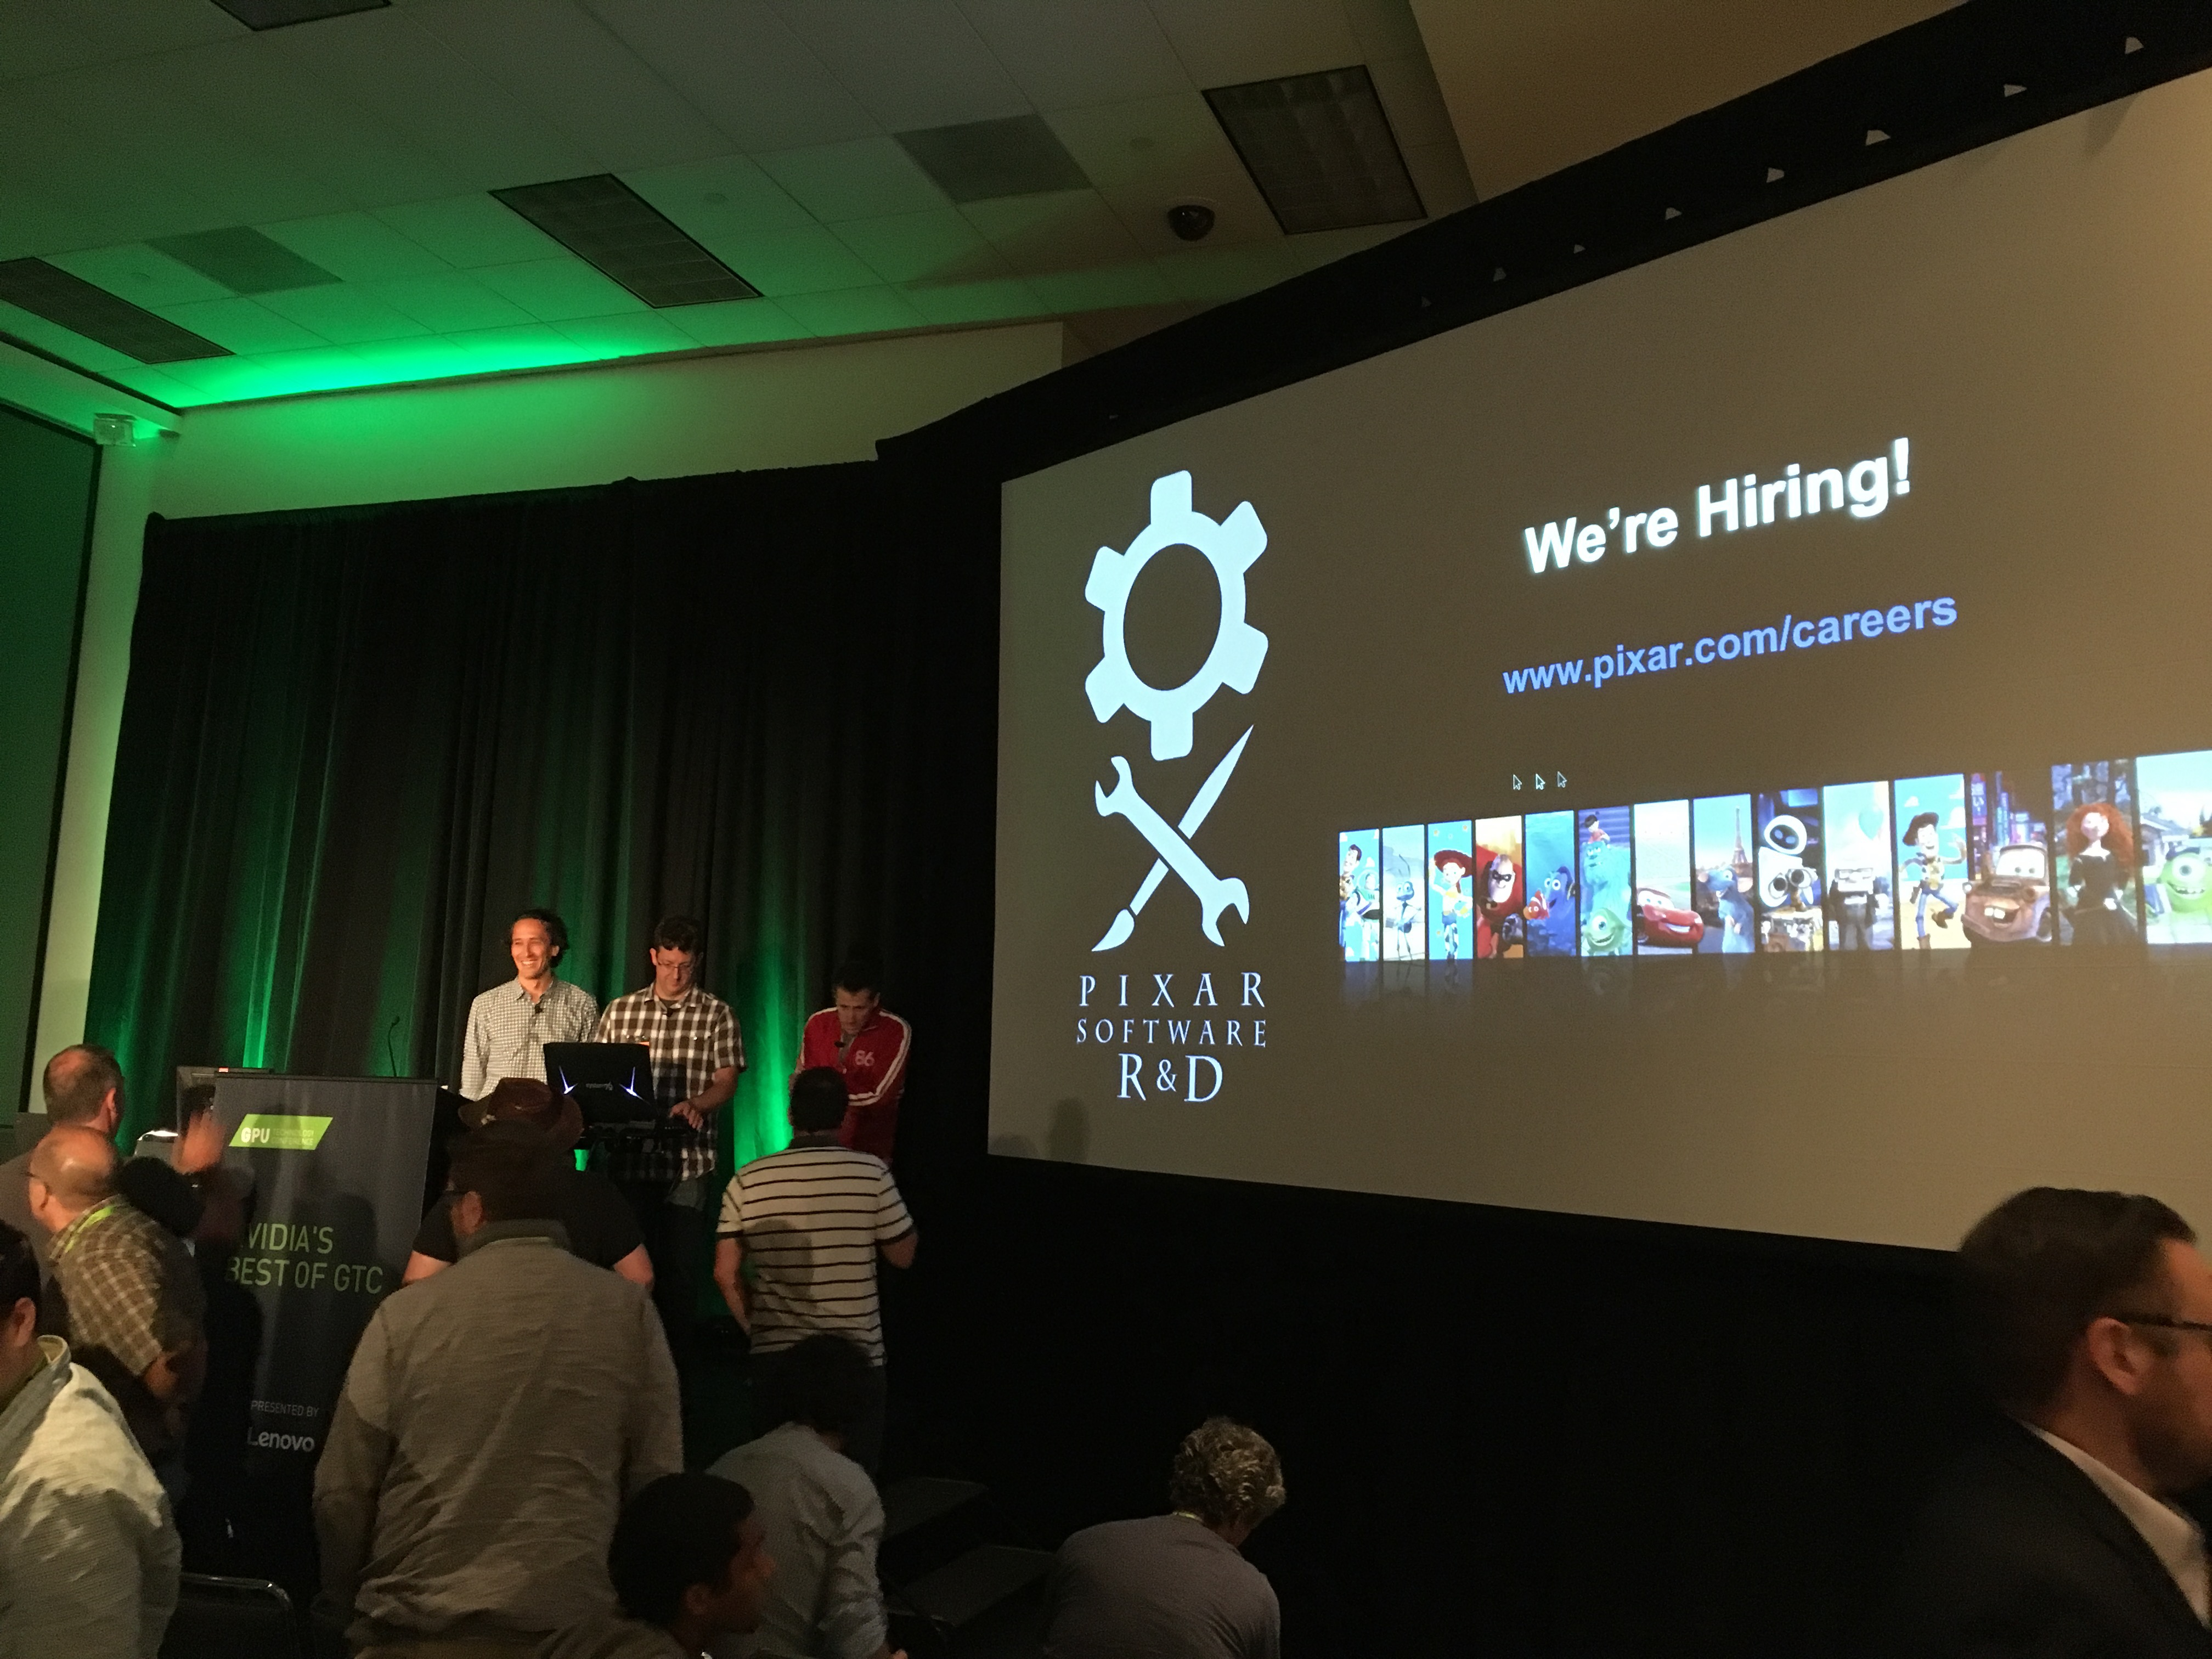
\includegraphics[width=\textwidth]{pixar_real-time}
	\caption*{\textit{NVIDIA Best of GTC Talks: Real-time Graphics for Film Production at Pixar}}
\end{figure}

One of the most impressive demos during the Pixar talk involved a rigged Lightning McQueen from \textit{Cars} whose face was manipulated in real-time in front of the audience. It was pointed out that riggers need to be able to operate on a smaller number of points than the ones produced in real-time by subdivision surfacing. You witness millions of triangles being blasted onto your screen as speaker  contorts Ligtning McQueen's face into a hilarious pout. "I'm not an animator," he says as the audience laughs.

You aren't quite sure what to see after the Pixar talk ends. After getting a bite to eat, you head to Hall B to see \textit{Technical Papers Fastforward}, a presentation from 6 to 8pm which gives speakers roughly one minute to talk (or stand silently) while their presentation plays out on a 30 foot screen. Each presenter alternates speaking at podiums on one side of the room so that while a presenter or group of researchers are talking, another presenter may prepare at the opposite podium. Some of the prsentations maintain an air of mystery about them, hinting at a worthwhile discussion of discrete differntial geometry to be had on such and such day at such and such time later in the week. Many of the presentations are tongue in cheek. Some of the most entertaining are the poorly translated videos which make use of an articicial intelligence system to bridge the language barrier. It's hard to know how competent these presentations will be when their one minute preview is similar to bad used car commercial. The guy from The Hebrew University of Jerusalem sitting next to you types each of these papers out on his laptop to keep track of the ones he would like to go listen to. You understand roughly 10 percent of what you hear and feel it will be worthwhile to attempt reading a few of the papers that are available online.

\begin{figure}[h!]
	\centering
	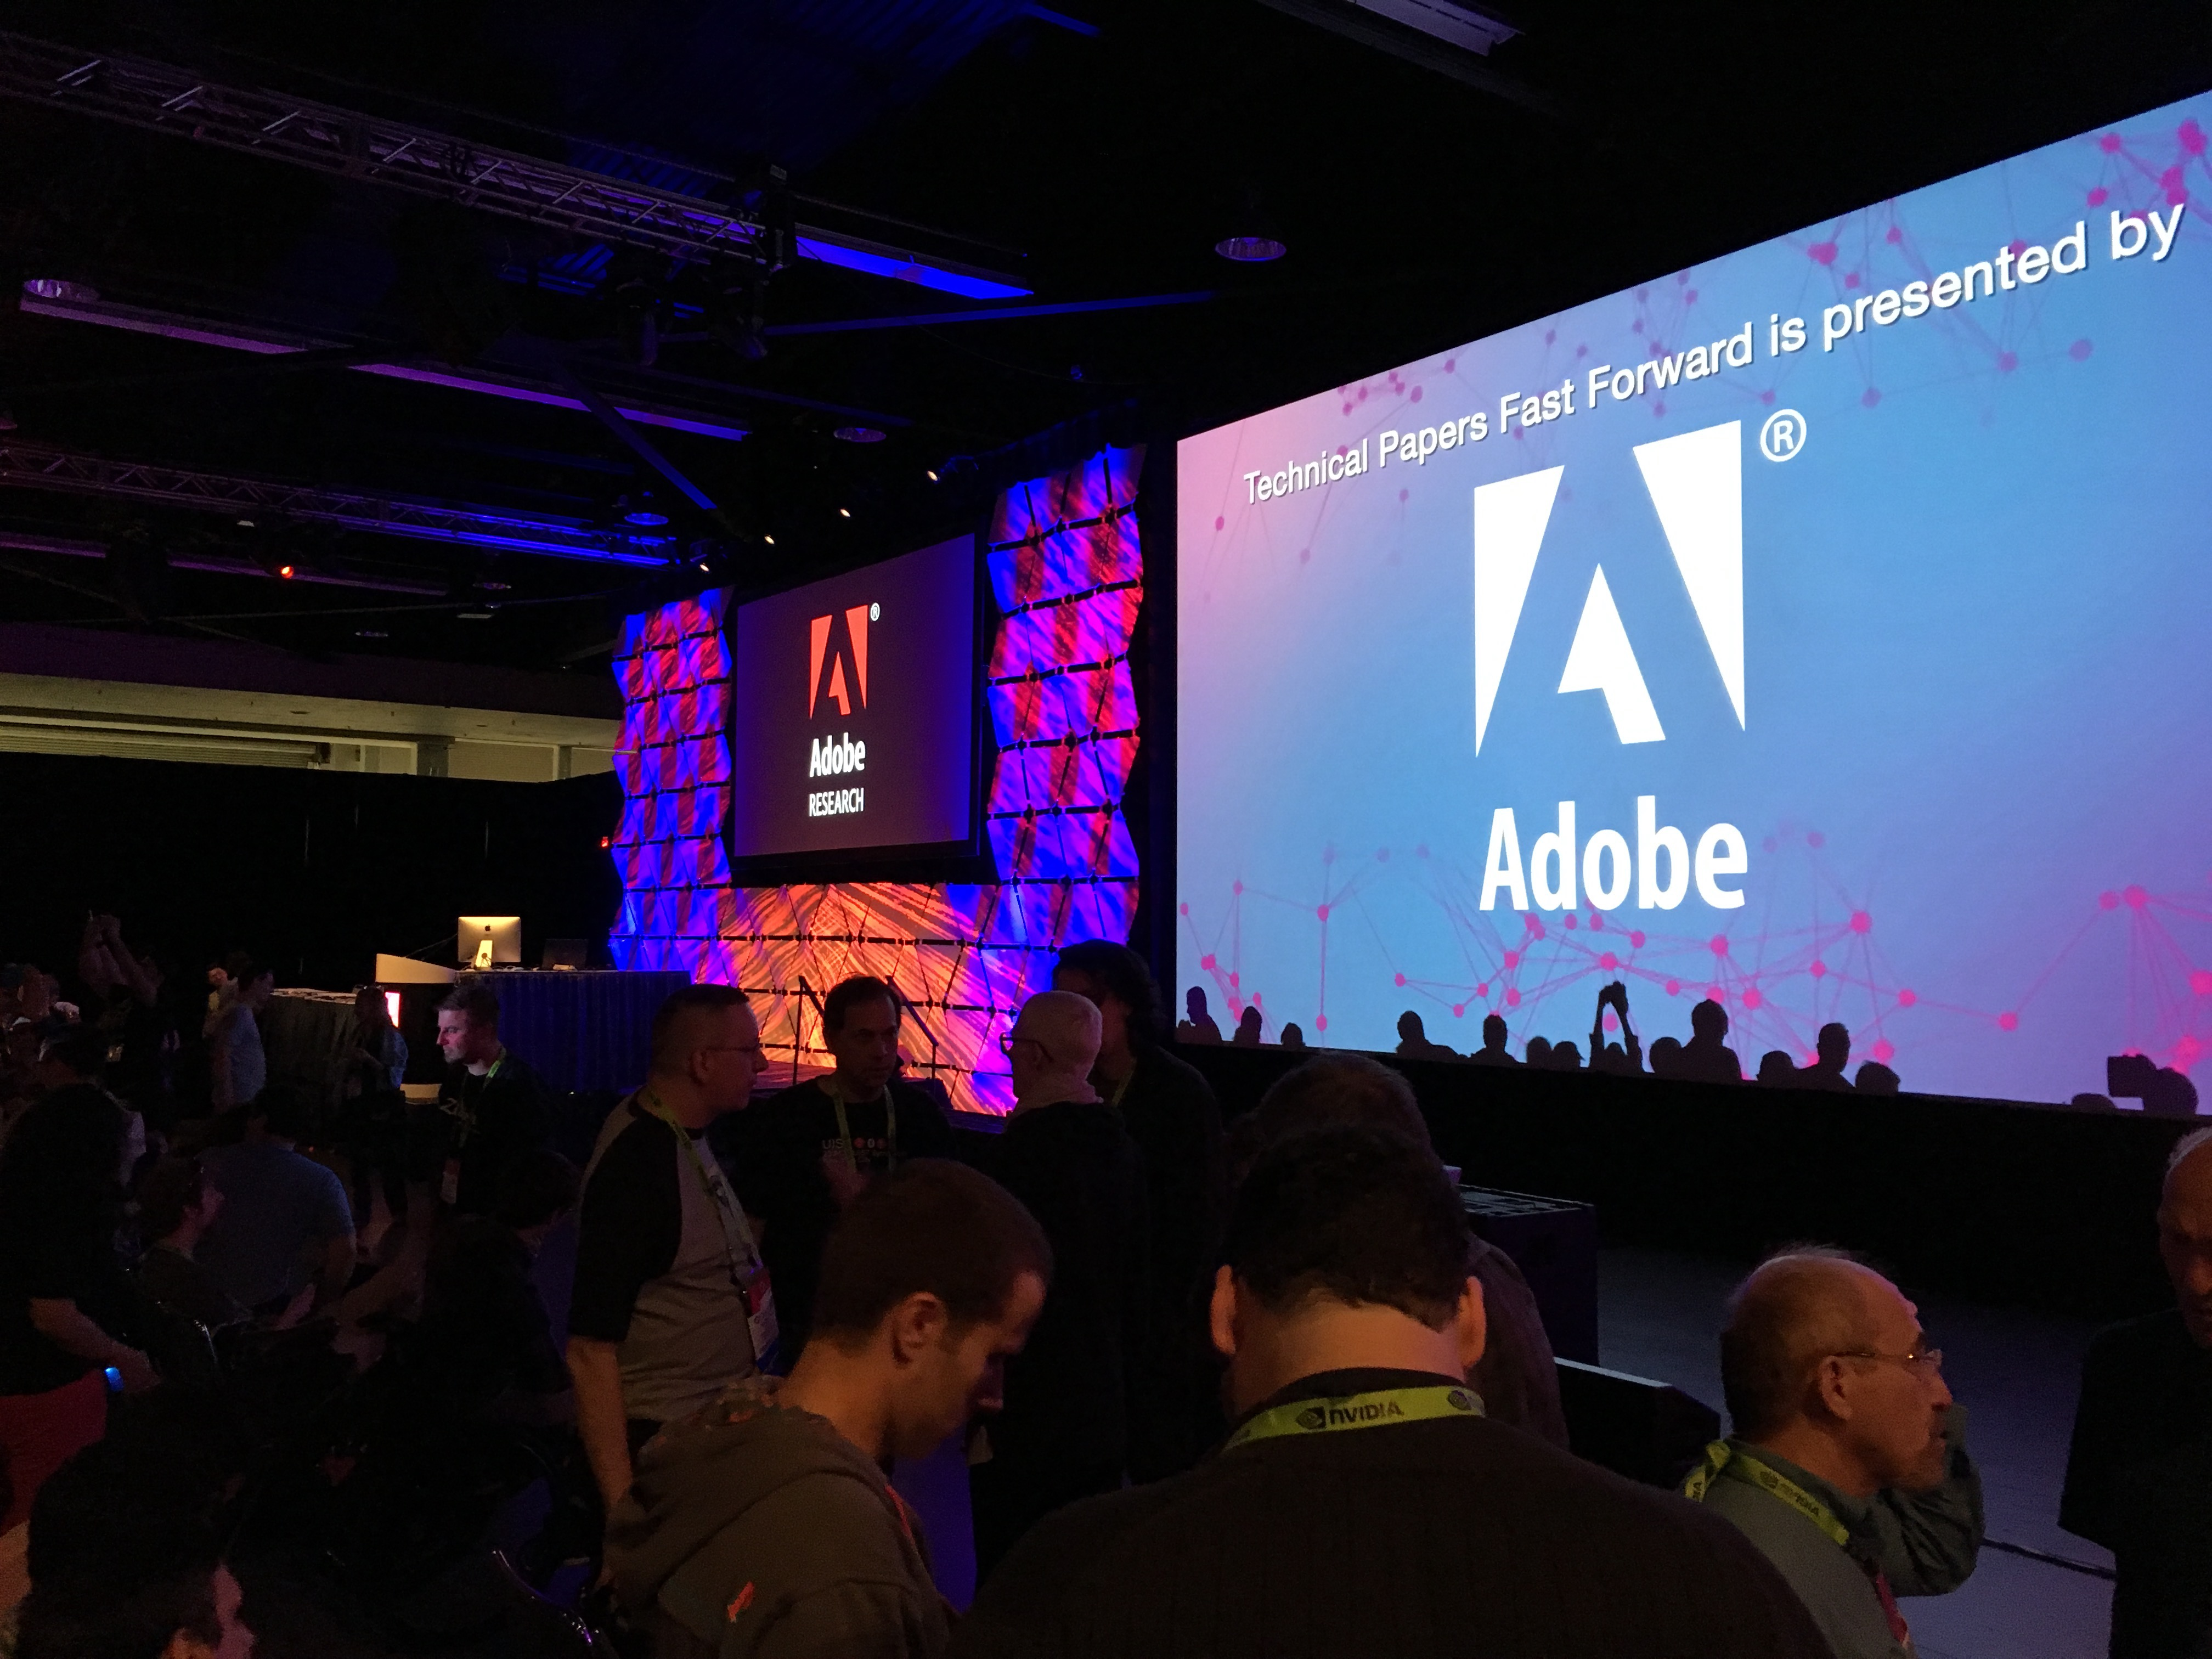
\includegraphics[width=\textwidth]{technical_papers}
	\caption*{Technical Papers Fast Forward, shown in Hall B}
\end{figure}

After the event, you meet up with your newfound crew and proceed to be driven around cramped in the back of a Chevy Sonic in seach of a place to eat. Despite your efforts to use Google Maps to find a walkable area to hang out with your new friends, you all wind up a few miles from the convention center at a greesy taco joint with green painted iron bars over the windows. It's decidedely \textit{not a nice part of town}, so you all eat and head to a sports bar where you finally have the chance to catch swap some stories and bond as recently graduated (or at least soon to be graduated) SVs. One girl is interning for Hasbro. Another is a student at School of the Arts Institute of Chicago. The third is a belgian student who just finished his technical training at a vocational school for game development in the Netherlands. The Belgian you find particularly entertaining; his articulate english delivered in a deep Dutch accent os not the least of his appeal as a cool cat within your group. He's funny and quite sharp, as are the others in your new SV crew. 

You are happy as you pitch in for a pitcher that you have started to make some friends. This feels like you are doing SIGGRAPH the right way, letting the information soak in and then reflecting on the day as you swap stories in the evening. After an hour or so you all part.

An Uber is hailed and you are soon heading home to post the day's pictures and check your schdule of shifts for tomorrow. You are asked to be respectful in not requesting shift swaps within 24 hours of your assigned time slot. Likewise, the SV committee tries their best not to swap your slots within this same courtesy window. It is entirely possible---likely, even---that the most important SIGGRAPH event, whatever you feel it may be, will coincide with a shift that you had not even seen when first checked your online portal on Sunday morning.

\end{document}